\cotefile{60}
\scanpage{2}

Notes sur \uline{l'équation fonctionnelle}

\margin{\unsure{b}}
\scanpage{3}

Si $f$ est un endomorphisme d'un vectoriel $E$ de dim finie $n$ sur le corps $k$, on pose
\[
\begin{aligned}
P_f(t)&=\det(1-ft)=\prod_i(1-\lambda_i t)\\
&=\sum_i(-1)^i(\operatorname{Tr}\lambda^i(f))t^i
\end{aligned}
\]
les $\lambda_i$ étant les \unsure{val.} propres dans une extension alg. close de $k$.

Donc les racines de $P_f(t)$ sont les inverses des valeurs propres non nulles de $f$.

$P_f(t)$ pour $(E,f)$ variable est ``additif'' en $E$ (suite exacte en $E$ \unsure{transformée} en produit des polynômes). Il en est de même de
\[
\begin{aligned}
Z_f(t)&=\frac{1}{P_f(t)}=\prod_i\frac{1}{1-\lambda_i t}=\prod_i\sum_{\nu}\lambda_i^{\nu}t^{\nu}\\
&=\sum_{\nu}t^{\nu}\sum_{\nu_1+\cdots+\nu_n=\nu}\lambda_1^{\nu_1}\cdots\lambda_n^{\nu_n}=\sum_{\nu}\operatorname{Tr}(\operatorname{Sym}^{\nu}(f))t^{\nu}.
\end{aligned}
\]

D'autre part, $P_f(t)$ transforme le produit tensoriel en $(E,f)$ en le ``produit'' $*$ des séries formelles commençant par $1$, où on a posé
\[
(1-at)*(1-bt)=1-abt
\]
[et distributivité de $*$ p.r. à $\cdot$, etc $\ldots$

\margin{\figure{
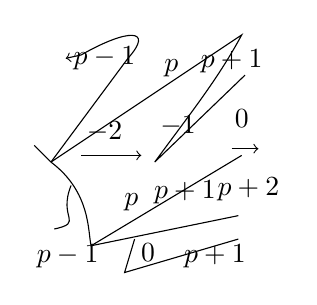
\begin{tikzpicture}[x=0.85cm,y=0.85cm]
\draw (0,1.55) -- (1.15,3.1) .. controls (1.55,3.55) and (1.15,3.55) .. (0.45,3.15);
\draw[->] (0.45,3.15) -- (0.22,3.1);
\draw (0,1.55) -- (2.85,3.45) .. controls (2.5,2.8) and (2.1,2.3) .. (1.55,1.55) -- (2.9,2.85);
\draw (0,1.55) -- (-0.25,1.8);
\draw (0,1.55) .. controls (0.6,1.1) and (0.55,0.5) .. (0.6,0.3) -- (2.85,1.65);
\draw (0.6,0.3) -- (2.8,0.75);
\draw (1.25,0.4) -- (1.1,-0.1) -- (2.8,0.4);
\draw[->] (0.45,1.65) -- (1.35,1.65);
\draw[->] (2.7,1.75) -- (3.1,1.75);
\node at (0.8,3.1) {$p-1$};
\node at (1.8,2.95) {\uline{$p$}};
\node at (2.7,3.05) {$\unsure{p+1}$};
\node at (0.8,2) {$-2$};
\node at (1.9,2.1) {$-1$};
\node at (2.85,2.2) {$0$};
\node at (1.2,0.95) {$p$};
\node at (2,1.1) {$\unsure{p+1}$};
\node at (2.95,1.15) {$\unsure{p+2}$};
\node at (0.25,0.15) {$p-1$};
\node at (1.45,0.2) {$0$};
\node at (2.45,0.15) {$p+1$};
\draw (0.3,1.2) .. controls (0.1,0.7) and (0.5,0.65) .. (0.05,0.55);
\end{tikzpicture}
}}

\mspage{2}
\scanpage{4}
\mspage{3}

\begin{center}- 57 -\end{center}
\margin{$\mathrm{n}^{\mathrm{o}}357$}

\[
f(x)\leq\sum_{i=1}^{n}a_i[\varphi(s_i)+\eta]g(s_i^{-1}x)
\]
et de même pour $f'$, et par suite :
\[
(f:g)+(f':g)\leq\sum_{i=1}^{n}a_i[\varphi(s_i)+\varphi'(s_i)+2\eta]\leq(1+2\eta)\sum_{i=1}^{n}a_i
\]
puisque $\varphi+\varphi'\leq1$. En appliquant la définition de $[F:g]$, puis (ii) et (vii), on en conclut :
\[
(f:g)+(f':g)\leq(1+2\eta)(F:g)\leq(1+2\eta)[(f+f':g)+\delta(h:g)]\ ;
\]
appliquant (v) à $f+f'$, $h$ et $g$, cela donne :
\[
(f:g)+(f':g)\leq(f+f':g)+2\eta(f+f':h)\cdot(h:g)+(1+2\eta)\delta\cdot(h:g).
\]
Si donc $f$, $f'$ et $h$ sont donnés comme dans (viii), il suffit de choisir $\delta$ et $\eta$ assez petits, puis de choisir $V$ comme il a été dit, pour qu'on ait l'inégalité formulée dans (viii).

Soit maintenant $\unsure{\mathfrak{F}|\mathcal{F}}$ un ultrafiltre sur $\mathcal{K}^{*}_{+}$, plus fin que le filtre engendré par la réunion des $\mathcal{K}^{*}_{+}(V)$ quand $V$ parcourt un système fondamental de voisinages compacts de $e$. D'autre part, fixons $f_0\in\mathcal{K}^{*}_{+}$ ; posons, pour $f\in\mathcal{K}^{*}_{+}$, $g\in\mathcal{K}^{*}_{+}$ :
\[
I_g(f)=\frac{(f:g)}{(f_0:g)},
\]
puis $I(f)=\lim_{\unsure{\mathfrak{F}|\mathcal{F}}}I_g(f)$. D'après (vi), $I(f)$ est dans l'intervalle $[1/(f_0:f),(f:f_0)]$. D'après (ii), on a $I(cf)=c.I(f)$ pour $c>0$. D'après (vii), on a $I(f+f')\leq I(f)+I(f')$. D'après (viii), on a $I(f+f')\geq I(f)+I(f')-\varepsilon I(h)$ quel que soit $\varepsilon\geq0$ si $h$ est $\geq1$ sur le support de $f+f'$ ; comme on peut toujours choisir $h$ ainsi dans $\mathcal{K}^{*}_{+}$, il s'ensuit que $I(f+f')=I(f)+I(f')$. Alors, d'après le Chap.II, § 2, n°1, prop.2, $I$ se prolonge (d'une manière et d'une seule) à une forme linéaire positive sur $\mathcal{K}$, c'est-à-dire qu'il y a une mesure positive $\alpha$ sur $G$ telle que $I(f)=\int f\,d\alpha$ pour $f\in\mathcal{K}^{*}_{+}$. D'après (i), on a $I(\gamma(\varepsilon_s)f)=I(f)$ quels que
\scanpage{5}

\[
\left\{\begin{aligned}
P_{f\otimes f'}(t)&=P_f(t)*P_{f'}(t)\\
L_{f\otimes f'}(t)&=\frac{1}{L_f(t)*L_{f'}(t)},
\end{aligned}\right.
\qquad L_{f_1\otimes\cdots\otimes f_{\nu}}(t)=\left(\prod L_{f_i}(t)\right)^{(-1)^{\nu+1}}
\]

De même, pour ``la'' $\lambda$-structure de $\unsure{1+k[[t]]^{+}}$ où $\deleted{\unsure{f}}\inserted{\lambda^p}$ transforme $\unsure{\widehat{\prod}_i|\prod_i}(1-\lambda_i t)$ en $\prod_{i_1<\cdots<i_p}(1-\lambda_{i_1}\cdots\lambda_{i_p}t)$, on aura
\[
\left\{\begin{aligned}
P_{\lambda^i f}(t)&=\lambda^iP_f(t),\qquad\text{donc}\\
\frac{1}{L_{\lambda^i f}(t)}&=\lambda^i\frac{1}{L_{\deleted{\unsure{\lambda}}f}(t)}
\end{aligned}\right.
\]
i.e.
\[
\begin{aligned}
-\sum\deleted{\unsure{1}}\inserted{(-1)^i}[L_{\lambda^i f}(t)]s^i
&=\lambda^*([-L_f(t)])(\unsure{-s|s})\\
&=\frac{1}{\lambda^*[L_f(t)](-s)}\deleted{(\unsure{-s})}
\end{aligned}
\]
\deleted{
\[
\left(\sum[\lambda^i(L_f(t))]s^i\right)\left(\sum[L_{\lambda^i f}(t)]s^i\right)=-1=\left[\frac{1}{1-t}\right]
\]
}
\[
=\sum\sigma^i(L_f(t))s^i
\]
\[
\left\{\begin{aligned}
L_{\lambda^i(f)}(t)&=\left(\sigma^i L_f(t)\right)^{(-1)^{i+1}}\\
L_{\sigma^i(f)}(t)&=\left(\lambda^i L_f(t)\right)^{(-1)^{i+1}}
\end{aligned}\right.
\]

\margin{\figure{\begin{tikzpicture}[x=1cm,y=1cm]\draw (0,.8) .. controls (-.15,1.2) and (-.12,1.5) .. (.03,1.4);\draw (0,.55) .. controls (.15,.3) and (.12,0) .. (.1,-.3);\end{tikzpicture}}}
\mspage{4}
\scanpage{6}
\mspage{5}

\begin{center}- 56 -\end{center}
\margin{$\mathrm{n}^{\mathrm{o}}357$}

\[
0<\frac{1}{(f_0:f)}\leq\frac{(f:g)}{(f_0:g)}\leq(f:f_0).
\]
\[
\text{(vii)}\qquad(f+f':g)\leq(f:g)+(f':g).
\]
(viii) si $f$, $f'$, $h$ sont dans $\mathcal{K}_+$, si $h\geq1$ sur le support de $f+f'$, et si $\varepsilon>0$, il y a un voisinage compact $V$ de $e$ tel que l'on ait, pour tout $g\in\mathcal{K}^*_+(V)$ :
\[
(f+f':g)\geq(f:g)+(f':g)-\varepsilon(h:g).
\]
Les trois premières sont évidentes ; (iv) aussi, puisque $\sup(\gamma(\mu)g)\leq\Vert\mu\Vert\sup(g)$ ; (v) résulte aussitôt de la formule $\Vert\mu*\mu'\Vert={} =\Vert\mu\Vert.\Vert\mu'\Vert$ (par la vertu du Chap.VII, § 1, n°1, ou, moins savamment et plus simplement dans le cas qui nous occupe ici, par un calcul direct trivial) et de ce qu'on a, si $f\leq\gamma(\mu)g$ et $g\leq\gamma(\mu')h$ :
\[
f\leq\gamma(\mu)\gamma(\mu')h=\gamma(\mu*\mu')h.
\]
Si on applique (v) à $f_0$, $f$, $g$ d'une part, et à $f$, $f_0$, $g$ d'autre part, on obtient (vi) ; (vii) est évidente. Enfin, soient $f$, $f'$, $h$ comme il est dit dans (viii). Posons $F=f+f'+\delta h$, avec $\delta>0$ ; les fonctions $\varphi$, $\varphi'$ qui coïncident respectivement avec $f/F$ et $f'/F$ sur le support de $f+f'$, et qui sont $0$ en dehors de celui-ci, sont dans $\mathcal{K}$, donc uniformément continues ; pour tout $\eta>0$, on peut donc choisir un voisinage compact $V$ de $e$ tel que $|\varphi(x)-\varphi(s)|$ et $|\varphi'(x)-\varphi'(s)|$ soient $\leq\eta$ pour $s^{-1}x\in V$ ; alors, quelle que soit $g\in\mathcal{K}^*_+(V)$, on aura
\[
\varphi(x)g(s^{-1}x)\leq[\varphi(s)+\eta]g(s^{-1}x)
\]
quels que soient $x$ et $s$, et de même pour $\varphi'$. Supposons maintenant qu'on ait, pour tout $x$ :
\[
F(x)\leq\sum_{i=1}^{n}a_i g(s_i^{-1}x).
\]
Puisque $f=\varphi F$, on en conclut :
\scanpage{7}

Considérons le cas d'un \uline{automorphisme} $f$, et voyons quel est le \unsure{polynôme} \unsure{du} contragrédient
\[
\begin{aligned}
P_{\check f}(t)&=\deleted{\det}(1-\check f t)=\prod(1-\lambda_i^{-1}t)\\
&\deleted{=\unsure{\prod}\lambda_i^{-1}(\lambda_i-t)}\\
&=\prod_i(-\lambda_i^{-1}t)(1-\lambda_i t^{-1})\\
&=\frac{(-1)^n t^n}{\prod\lambda_i}\deleted{\unsure{\det}}\prod(1-\lambda_i t^{-1})\\
&=\frac{(-1)^n t^n}{\det f}P_f(\unsure{-t^{-1}|t^{-1}})
\end{aligned}
\]
donc
\deleted{
\[
P_{\check f}(t)=\deleted{\frac{\unsure{(-1)^n t^n}}{\det f}}\unsure{\varepsilon(f)}t^nP_f(t^{-1})\qquad\unsure{\varepsilon(f)}=
\]
}
\[
\boxed{P_{\check f}(t)=(-t)^{\varepsilon(f)}\det f^{-1}\,P_f(t^{-1})}
\]
i.e
\[
\boxed{L_{\check f}(t)=(-t)^{-\varepsilon(f)}\det f\,L_f(t^{-1})}
\]
Bien entendu, la dernière n'a \unsure{pas} de sens quand on \unsure{substitue|remplace} $\unsure{P_f^{\pm}(t)|P_f(t)}$ par une série formelle quelconque : il est essentiel de se borner aux séries formelles qui sont produits \unsure{alternés} finis de \uline{polynômes} [à terme constant $1$, à terme dominant inversible -- cette dernière condition n'étant utile que si $k$ est un anneau \unsure{général|quelconque} $\ldots$].

\mspage{6}
\scanpage{8}
\mspage{7}

\begin{center}- 55 -\end{center}
\margin{$\mathrm{n}^{\mathrm{o}}357$}

[N.B. -- Ce n'est pas par amour des méthodes éculées et pisseuses que le rédacteur, dans la construction de la mesure de Haar, est revenu aux mesures à support \uline{fini} au lieu des mesures à support \uline{compact} des rédactions précédentes ; c'est en vertu du rasoir d'Occam (``entitates non sunt multiplicandae''), et pour pouvoir laisser reposer en paix dans la Remarque de la fin du Chap.VII, § 2, n°2, la théorie générale de l'opération $\mu*f$, ou $\gamma(\mu)f$, lorsqu'on ne s'est pas donné de jauge ; ce n'est évidemment pas difficile (cf. loc. cit.), mais ça paraît bien superflu $\ldots$]

On écrira $\mathcal{K}$, $\mathcal{K}(K)$, etc. au lieu de $\mathcal{K}(G)$, $\mathcal{K}(G,K)$, etc. ; on notera $\mathcal{K}_+$ l'ensemble des fonctions $f\in\mathcal{K}$ à valeurs $\geq0$, $\mathcal{K}^*_+$ l'ensemble des fonctions $g\in\mathcal{K}_+$ autres que $0$, et $\mathcal{K}^*_+(K)$, si $K$ est une partie compacte de $G$, l'ensemble des fonctions $g\in\mathcal{K}^*_+$ à support contenu dans $K$. Pour $f\in\mathcal{K}_+$, $g\in\mathcal{K}^*_+$, désignons par $A(f,g)$ l'ensemble des mesures positives $\mu\neq0$, à support fini, telles que $f\leq\gamma(\mu)g$. \uline{Cet ensemble n'est pas vide.} En effet, soient $K$ le support de $f$, et $U$ un ouvert non vide tel que $m=\inf_U(g)>0$ ; soit $M=\sup_K(f)$. On peut recouvrir $K$ par un nombre fini d'ensembles $s_iU$ ; alors la mesure $(M/m)\sum\varepsilon_{s_i}$ est dans $A(f,g)$. Posons maintenant :
\[
(f:g)=\inf_{\mu\in A(f,g)}\Vert\mu\Vert.
\]
Il est clair qu'on a $0\leq(f:g)<+\infty$. De plus, ce symbole a les propriétés suivantes :

(i) $(\gamma(\varepsilon_s)f:g)=(f:g)$ quel que soit $s\in G$.

(ii) $(cf:g)=c.(f:g)$ quel que soit $c\geq0$.

(iii) $f\leq f'$ entraîne $(f:g)\leq(f':g)$.

(iv) $(f:g)\geq(\sup f)/(\sup g)$.

(v) $(f:h)\leq(f:g).(g:h)$ pour $g\in\mathcal{K}^*_+$, $h\in\mathcal{K}^*_+$.

(vi) si $f$, $f_0$, $g$ sont dans $\mathcal{K}^*_+$, on a :
\scanpage{9}

Si $E$ est un \deleted{motif} \inserted{$\mathbb{Q}_{\ell}$-faisceau} sur $\unsure{\operatorname{Sp}|\operatorname{Spec}}\mathbb{F}_p$, \deleted{\unsure{donc}} on trouve donc
\[
L_{\check E}(t)=(-t)^{-n}\det f_E\,L_E(t^{-1})
\]
où $n=\operatorname{rang}E$ et s'il s'agit d'un \uline{motif} \inserted{de poids $\rho$} satisfaisant aux conj. de Weil
\[
\left\{\det f_E=\deleted{\varepsilon}\inserted{\varepsilon(E)}p^{\frac{n\rho}{2}}\right.
\]
avec $\varepsilon=\pm1$ [dépendant du motif $\bigwedge^n E$, \unsure{suivant|savoir} si $f$ y opère \unsure{positivement} ou non] ; noter que $\frac{n\rho}{2}$ est tjrs entier (i.e. $\rho$ impair $\Longrightarrow n$ pair).

On trouve donc
\[
L_{\check E}(t)=\varepsilon(E)(-p^{\rho/2}/t)^n L_E(t^{-1}).
\]

D'autre part, par Lefschetz, on aura
\[
\check E\simeq E(\rho)
\]
d'où
\[
\begin{aligned}
L_{\check E}(t)&=\left(L_E(t)*L_{\mathbb{Q}_{\ell}(\rho)}(t)\right)^{-1}\\
&=\left(L_E(t)*\frac{1}{1-p^{-\rho}t}\right)^{-1}=L_E(t)*(1-p^{-\rho}t)
\end{aligned}
\]
\[
L_{\check E}(t)=L_E\left(\frac{t}{p^{\rho}}\right)
\]

\mspage{8}
\scanpage{10}
\mspage{9}

\begin{center}
CHAPITRE VIII

CONS\unsure{T}RUCTION de MESURES INVARIANTES

§ 1. \uline{Construction d'une mesure de Haar.}
\end{center}

\uline{Dans ce} §, $G$ \uline{désignera un groupe localement compact}.

1. \uline{Le théorème d'existence et d'unicité}.

Rappelons (Chap.VII, § 2, n°4) qu'on appelle \uline{mesure de Haar} sur $G$ toute mesure positive $\alpha\neq0$ sur $G$, invariante à gauche, et qu'une telle mesure est alors une jauge propre à gauche et à droite, satisfaisant à une formule de la forme
\[
d\alpha(axb)=\Delta_G(b)d\alpha(x)
\]
quels que soient $a\in G$, $b\in G$, $\Delta_G$ étant un caractère de $G$ ; on a alors
\[
d\alpha(x^{-1})=\Delta_G(x^{-1})d\alpha(x).
\]
Si $\Delta_G=1$, $\alpha$ est invariante à gauche et à droite ; on dit que $\alpha$ est \uline{bi-invariante} ; il en est évidemment ainsi si $G$ est commutatif.

THEOREME 1.-- \uline{Sur tout groupe localement compact} $G$, \uline{il existe une mesure de Haar, et, à un facteur constant près, il n'en existe qu'une}.

L'unicité a déjà été démontrée (Chap.VII, § 2, n°4, th.1) ; on va démontrer l'existence par une construction explicite. Introduisons d'abord une notation. Soit $\mu=\sum_{i=1}^{n}a_i\varepsilon_{s_i}$ une mesure de support fini $\{s_1,\ldots,s_n\}$ sur $G$ ; alors, pour $f\in\mathcal{K}(G)$, on désignera par $\gamma(\mu)f$ la fonction $f'\in\mathcal{K}(G)$ définie par
\[
f'(x)=\sum_{i=1}^{n}a_i f(s_i^{-1}x)\ ;
\]
\margin{\figure{\begin{tikzpicture}[x=1cm,y=1cm]
\draw (0,2.5) .. controls (0.7,2.65) and (1.3,2.05) .. (0.85,2.2);
\draw (0.15,1) .. controls (1.5,0.8) and (1.35,0.55) .. (0.2,0);
\end{tikzpicture}}}

on notera que, dès qu'on aura construit une mesure de Haar, on aura le droit, en vertu des définitions du Chap.VII, § 2, d'écrire $\mu*f$ au lieu de $\gamma(\mu)f$ (cf. la Remarque à la fin du Chap.VII, § 2, n°2). L'application $(\mu,f)\longrightarrow\gamma(\mu)f$ ainsi définie est évidemment bilinéaire ; comme on a $\gamma(\varepsilon_{st})=\gamma(\varepsilon_s)\gamma(\varepsilon_t)$, on en conclut qu'on a $\gamma(\mu*\nu)=\gamma(\mu)\gamma(\nu)$. De plus, $\gamma(\mu)f$ est $\geq0$ si $\mu$ et $f$ sont $\geq0$ ; et, si $\mu$ et $f$ sont $\geq0$, on ne peut avoir $\gamma(\mu)f=0$ que si $\mu=0$ et $f=0$.
\scanpage{11}

On trouve donc
\[
\boxed{L_E\left(\deleted{\unsure{t^{-1}}}\frac{1}{tp^{\rho}}\right)=\deleted{\unsure{(-t)^n}}\det f_E(-t)^nL_E(t)}
\]
[$\rho$ étant le poids de $E$, qui s'introduit via $\check E\simeq E(\rho)$]

\figure{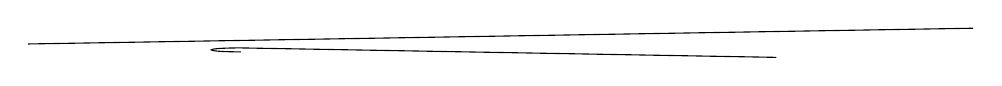
\begin{tikzpicture}[x=1cm,y=1cm]
\draw (0,0.25) -- (12,0.45);
\draw (2.7,0.15) .. controls (2.2,0.15) and (2.2,0.2) .. (2.7,0.2) -- (9.5,0.08);
\end{tikzpicture}}

Soit $E$ un $\mathbb{Q}_{\ell}$-faisceau constructible sur $X$ \deleted{compactifiable} \inserted{propre} sur $\mathbb{F}_p$, alors on aura
\deleted{
\[
H_c^i(X,DE)\simeq D(H^{-i}(X,E))
\]
}
par le th. de dualité globale
\deleted{d'où donc
\[
\chi(DE)=\sum(-1)^iH^i(X,D(E))\simeq D(\chi(E))
\]
}
\[
\mathbf{R}f_*(DE)=D(\mathbf{R}f_*(E))
\]
d'où
\[
\left\{\begin{aligned}
&\text{(1)}\quad\boxed{L_{DE}(t)=(-t)^{-\chi(E)}\delta(E)\,L_E(t^{-1})}\\
&\chi(E)=\operatorname{rang}\mathbf{R}f_*E=\sum(-1)^i\operatorname{rg}H^i(\bar X,\bar E)\\
&\delta(E)=\prod_i\left(\det f_{H^i(\bar X,\unsure{\bar F|\bar E})}\right)^{(-1)^i}=\varepsilon(E)p^{\sum_i(-1)^i\deleted{\unsure{\rho}}\frac{i+\rho}{2}b_i}
\end{aligned}\right.
\]
\inserted{avec les conjectures \unsure{standart|standard}, si $X$ est \deleted{\unsure{projectif|propre}} \inserted{lisse purement de dim $n$} \deleted{lisse} et $F$ \unsure{c$^{\mathrm{t}}$|c.t.} tordu \unsure{purement} de poids $\rho$}
\margin{invariant géométrique}
\margin{invariant arithmétique}
\margin{$b_i=\operatorname{rang}H^i(\bar X,\bar F)$}

\mspage{10}
\scanpage{12}

\begin{center}- 2 -\end{center}
\margin{$\mathrm{n}^{\mathrm{o}}398$}

PROPOSITION 2.-- \uline{Si} $E'\longrightarrow E\longrightarrow E''$ \uline{est une suite exacte de} $A$-\uline{modules de longueur finie, la suite} $E''^*\longrightarrow E^*\longrightarrow E'^*$ \uline{est exacte}.

Soit d'abord $0\longrightarrow L\longrightarrow M\longrightarrow N\longrightarrow0$ une suite exacte de modules de longueur finie et montrons que $0\longrightarrow N^*\longrightarrow M^*\longrightarrow L^*$ est exacte. C'est en tout cas vrai pour $0\longrightarrow N^*\longrightarrow M^*\longrightarrow L^*$, d'après les propriétés générales de $\operatorname{Hom}$. Comptant les longueurs, on en déduit que $M^*\longrightarrow L^*$ est surjectif, d'où le résultat.

Le cas d'une suite exacte qqe $E'\longrightarrow E\longrightarrow E''$ se ramène au précédent en dévissant à la façon habituelle, (Chap. II, 3e éd., p. 21). Soit $E$ un $A$-module. Si $F\subset E$, on note $F^{\circ}$ son orthogonal dans $E^*$, i.e. etc $\ldots$

PROPOSITION 3.-- \uline{Soit} $E$ \uline{un} $A$-\uline{module de longueur finie}. \uline{La correspondance qui à} $F\subset E$ \uline{fait correspondre} $F^{\circ}$ \uline{est une bijection de l'ensemble des sous-modules de} $E$ \uline{sur celui des sous-modules de} $E^*$ ; \uline{cette bijection transforme somme en intersection et intersection en somme}.

On utilise la suite exacte $0\longrightarrow(E/F)^*\longrightarrow E^*\longrightarrow F^*\longrightarrow0$, qui montre que $F^*$ s'identifie à $E^*/F^{\circ}$ et $(E/F)^*$ à $F^{\circ}$. On en déduit que l'injection $F\longrightarrow F^{\circ\circ}$ s'identifie à l'injection $F\longrightarrow F^{**}$, qui est un isomorphisme. D'où, etc $\ldots$

\uline{Exemple}.-- $A=$ \uuline{$Z$}, $K/A=$ \uuline{$Q$}$/$\uuline{$Z$} ; on a une dualité pour les groupes abéliens finis.

\begin{center}-:-:-:-\end{center}

\mspage{11}
\scanpage{13}
Dans ce cas favorable
\diagram{\begin{tikzcd}[ampersand replacement=\&,column sep=0.2em,row sep=1.4em]
\displaystyle\sum_i(-1)^i\frac{i+\rho}{2}b_i=\frac{\rho}{2}\chi(E)+\frac12 \& \displaystyle\underbrace{\sum_{i=0}^{2n}(-1)^i i b_i} \arrow[d,no head] \\
\& \displaystyle\sum_{i=0}^{n-1}\left[(-1)^i i b_i+(-1)^{2n-i}(2n-i)b_{2n-i}\right]+(-1)^n n b_n
\end{tikzcd}}
comme $b_i=b_{2n-i}$
\[
2n\sum_{i=0}^{n-1}(-1)^i b_i+(-1)^n n b_n=n\sum_{i=0}^{2n}(-1)^i b_i=n\chi(E)
\]
\[
\sum_i(-1)^i\frac{i+\rho}{2}b_i=\deleted{\unsure{n+\rho}}\frac{n+\rho}{2}\chi(E)
\]
donc
\[
\delta(E)=\unsure{\varepsilon(E)|\delta(E)}p^{\frac{n+\rho}{2}\chi(E)}
\qquad\varepsilon(E)=\pm1
\]
Par suite l'équation fonctionnelle devient dans ce cas
\[
(\unsure{2|1})\qquad L_{DE}(t)=\varepsilon(E)\left(-p^{\frac{n+\rho}{2}}\frac1t\right)^{\chi(E)}L_E(t^{-1}).
\]
Ou encore, si on admet que
\[
\check E\deleted{\unsure{DE}}\simeq E(\rho)
\]
globalement sur $X$ \deleted{\unsure{alors}}
\inserted{[il suffit que ce soit vrai sur le corps des fonctions de $X$, \unsure{donc c'est bon, donc tjrs vrai}]}
\[
\deleted{\unsure{L_E}}D(E)\simeq\deleted{\unsure{\check E\otimes\mathbb Q_\ell(n)}}\check E(n)[2n]\simeq E(\rho+n)[2n].
\]
\margin{\diagram{\begin{tikzcd}[ampersand replacement=\&,column sep=6em,row sep=0.4em]
{[2n]}\arrow[d,no head] \& {[2n]}\arrow[d,no head]\\
\text{shift} \& \text{shift}
\end{tikzcd}}}
et par suite
\[
\deleted{L_{DE}\simeq L_{E(\rho+n)}=L_{\mathbf R f_*(E(\rho+n))}}
\]
\[
\mathbf R f_*(D(E))\simeq\mathbf R f_*(E)(\rho+\deleted{2}n)[2n]
\]
d'où
\[
L_{DE}(t)=L_{\mathbf R f_*D(E)}(t)\simeq L_{\mathbf R f_*(E)}\left(p^{-(\rho+n)}t\right).
\]
\deleted{et il vient}
\mspage{12}
\scanpage{14}
\begin{center}- 9 -\end{center}
\hfill n° 57

\uline{Espace des sous-groupes fermés}, (n° 384)

C'est adopté, et ça ira en § 5 du chap. VIII d'Intégration. On vide l'espace uniforme des parties fermées et la prop. 3 (passent en exerc., avec appel d'exerc.).

Godement a fait une nouvelle rédaction en Congrès, qui a été relue, et améliorée quant aux virgules ; le rédacteur définitif a noté celles-ci.

\uline{Ce qui devrait être le chapitre des groupes de Lie} (n° 385 et 386).

Le n° 385 (``Distributions ponctuelles sur une variété''), sera incorporé dans le Fasc. Rés. des Variétés, après avoir été considérablement allégé. On n'y parlera pas du cas algébrique (ce qui simplifie en bas de la p. 3, le corps étant infini). Naturellement, ça doit être refondu avec les jets. On dira ``distributions à support fini''. Alléger les sorites (p. ex. celui des produits, n° 8 ; pourquoi pas les limites inductives et projectives ??).

L'énorme n° 386 (``Groupes formels et hyperalgèbres'') n'est pas du tout ce que Bourbaki voulait. D'une part le lien entre groupes analytiques et algèbres de Lie n'est fait que dans un mythique chapitre ultérieur. D'autre part on n'y démontre pas de résultats substantiels sur les groupes formels en caract. $p$. Ainsi Bourbaki vide toute la rédaction, et, comme Edith Piaf, ``on repart à zéro''. Cependant, le § 4 prévu par Cartier (correspondance entre groupes formels et algèbres de Lie en caract. 0, formule de Hausdorff), nettement plus substantiel que le reste, devra être rédigé pour usage ultérieur.

Là dessus Bourbaki s'aperçoit qu'il dispose d'une fort bonne rédaction de Koszul (``Variétés de groupes'', n° 340), sur laquelle on a intelligemment travaillé (voir Tribu n° 51). Ça doit facilement s'articuler avec le Fasc. Rés. Variétés. Bruhat devra rédiger sur cette base, sans chercher à faire d'originalité. Sinon le Livre de Lie est fichu !

\begin{center}-:-:-:-\end{center}
\begin{center}\uline{Séminaire BOURBAKI}\end{center}
Décembre 62 :

\diagram{\begin{tabular}{ll}
CARTIER & -- Fluctuations dans les suites de variables aléatoires indépendantes\\
\unsure{DEJHAN} & -- Papier Gårding à la S. M. F.\\
DIEUDONNÉ & -- Travail de Kostant (sur Amitsur -- \ldots{} etc)
\end{tabular}}
\mspage{13}
\scanpage{15}
\[L_{DE}(t)=L_E\left(p^{-(n+\rho)}t\right)\]
d'où, portant dans (2) et remplaçant $t$ par $t^{-1}$ :
\[
(3)\qquad\boxed{L_E\left(\frac1{p^{n+\rho}t}\right)=\varepsilon(E)\left(-p^{\frac{n+\rho}{2}}t\right)^{\chi(E)}L_E(t)}
\]
Posant
\[\boxed{\unsure{\xi|\zeta}_E(t)=t^{\chi(E)/2}L_E(t)}\]
il vient l'équation fonctionnelle
\[\boxed{\unsure{\xi|\zeta}\left(\frac1{p^{n+\rho}t}\right)=\varepsilon'(E)\unsure{\xi|\zeta}(t)}\]
\[
\begin{aligned}
\varepsilon'(E)&=\pm1,\qquad\varepsilon'(E)=(-1)^{\chi(E)}\prod_i\operatorname{signe}\det f_{H^i(\bar X,\bar F)}\\
&\hspace{7em}=(-1)^{\chi(E)}\operatorname{signe}\det f_{H^*(\bar X,\bar F)}
\end{aligned}
\]
\deleted{Si on écrit l'équation fonctionnelle avec $\varepsilon(E)$ au lieu de}

Notons d'ailleurs que $H^i(\bar X,\bar E)$ et $H^{2n-i}(\bar X,\check{\bar E})$ \inserted{$\simeq H^{2n-i}(\bar X,\bar E(\rho))=H^{2n-i}(\bar X,\bar E)(\rho)$} étant ``duaux à valeurs dans $\mathbb Q_\ell(n)$'', et l'opération de $f$ sur \inserted{$\mathbb Q_\ell(n)$} \unsure{ce dernier positive},
\[\varepsilon_i(E)=\varepsilon_{2n-i}(E),\]
et par suite on trouve que
\[\boxed{\varepsilon(E)=\operatorname{Signe}\det f_{H^n(\bar X,\bar E)}}.\]
\unsure{Pour la raison analogue}, $(-1)^{\chi(E)}=(-1)^{b_n}$. Donc
\[\varepsilon'(E)=(-1)^{b_n(E)}\operatorname{signe}\det f_{H^n(\bar X,\bar E)}.\]
\mspage{14}
\scanpage{16}
\hfill Rédaction n° 398
\begin{center}
COMPLÉMENTS AU CHAPITRE VII D'ALGÈBRE

DUALITÉ DES MODULES DE LONGUEUR FINIE SUR UN ANNEAU PRINCIPAL

-:-:-:-

CONTRE-RÉDACTION
\end{center}

[On se refuse à parler de modules injectifs, et d'autre part on se borne aux modules de longueur finie. Cela donne une rédaction minimale, (dans l'ensemble des rédactions $\neq\varnothing$)].

\uline{Notations}.

$A$ désigne un anneau principal, $K$ son corps des fractions. On suppose $K\neq A$ : i.e., $A$ possède au moins un élément extrémal.

Si $E$ est un $A$-module, on pose $E^*=\operatorname{Hom}(E,K/A)$ ; c'est un $A$-module. A tout homomorphisme $E\longrightarrow F$ correspond un homomorphisme $F^*\longrightarrow E^*$. Si $x\in E$, $x^*\in E^*$, on pose $x^*(x)=(x,x^*)$. On définit ainsi une application $A$-bilinéaire de $E\times E^*$ dans $K/A$, d'où un homomorphisme :
\[i_E:E\longrightarrow E^{**}.\]

PROPOSITION 1.- \uline{Si} $E$ \uline{est un} $A$-\uline{module de longueur finie}, $E^*$ \uline{est isomorphe}, (non canoniquement en général), \uline{à} $E$, \uline{et l'application} $i_E:E\longrightarrow E^{**}$ \uline{est un isomorphisme}.

Vu les théorèmes de structure, on peut se borner au cas où $E=A/tA$, avec $t\neq0$. Dans ce cas $E^*$ s'identifie au sous-module de $K/A$ formé des $x$ tels que $tx=0$, i.e. au sous-module $t^{-1}A/A$, isomorphe à $A/tA$. D'où l'isomorphie de $E$ et de $E^*$. Enfin, lorsque $E=A/tA$, la détermination précédente montre que $E^{**}$ s'identifie à $A/tA$ et l'on vérifie tout de suite que, dans ce cas, $i_E$ est l'application identique. D'où la deuxième partie de la proposition.
\mspage{15}
\scanpage{17}
\uline{Si} $n+\rho$ \uline{est impair}, alors $b_n=\dim\underbrace{H^n(\bar X,\bar E)}_{\text{poids }n+\rho}$ est pair, donc $\deleted{\unsure{\varepsilon}}(-1)^{b_n}=1$. De plus, un raisonnement du cours de \unsure{Serre} utilisant une forme alternée non dégénérée \unsure{invariante} montre que dans ce cas $\operatorname{signe}\det f_{H^n(\bar X,\bar E)}$ est égal à $+1$. Donc on trouve alors $\varepsilon'(E)=1$.

Si $n+\rho$ est pair, on ne peut déterminer le signe de façon absolue. On peut \deleted{\unsure{seulement affirmer que}} \margin{(\unsure{analogue de la parité|anal. de la parité})}
si $\unsure{\varepsilon_1|e_1}$ ($\unsure{\varepsilon_{-1}|e_{-1}}$) est \unsure{la} \deleted{\unsure{dimension}} \inserted{multiplicité} de \deleted{\unsure{l'espace}} la valeur propre $1$ ($-1$) de $f$ sur $H^n(\bar X,\bar F)$, on a
\[
(-1)^{b_n}=(-1)^{\unsure{\varepsilon_1+\varepsilon_{-1}|e_1+e_{-1}}},\qquad\varepsilon(E)=(-1)^{\unsure{\varepsilon_{-1}|e_{-1}}},
\]
donc
\[\boxed{\varepsilon'(E)=(-1)^{\unsure{\varepsilon_1|e_1}}}.\]

Lorsque l'on n'est pas dans le cas favorable $X$ lisse, $E$ \unsure{c$^{\mathrm{t}}$|ct} \unsure{tordu}, $\deleted{\unsure{E}}\check E$ \uline{globalement} isomorphe à $E(\rho)$, alors $D(E)$ ne s'exprime plus de façon aussi simple en fonction de $E$, et l'équation fonctionnelle (1) ne s'exprime plus \unsure{nec.|avec} en termes de la seule fonction $L_E$ [mais elle relie \uline{deux} fonctions $L_{DE}$, $L_E$]
\mspage{16}
\scanpage{18}
\begin{center}- 8 -\end{center}
\hfill n° 57

\diagram{\begin{tabular}{|lcl|}\hline
DIEUDONNÉ & : & \shortstack[l]{Rédactions définitives\\Systèmes de Racines (Juin 63)}\\\hline
DIXMIER & : & Théorie fine des algèbres normées (mars 63)\\\hline
GODEMENT & : & Rapport d'Analyse dirigée vers les groupes semi-simples (Juin 63)\\\hline
KOSZUL & : & Géométrie Riemannienne locale et globale (Juin 63)\\\hline
LANG & : & Rapport sur Mlle Bastiani \margin{?}\\\hline
SAMUEL & : & La Tribu\\\hline
SCHWARTZ & : & Rapport sur les Probas (?)\\\hline
SERRE & : & \shortstack[l]{Semi-simples complexes (Juin 63)\\Papier sur l'approximation forte dans SL}\\\hline
TATE & : & Dimension (mars 63),\\\hline
WEIL & : & Rien\\\hline
\end{tabular}}

\begin{center}-:-:-\end{center}
\begin{center}\uline{DÉCISIONS LOCALES DIVERSES}\end{center}
\uline{Errata}.

Pour Ens. III, p. 26 : remplacer ``\unsure{filrtant|filtrant} à droite et à gauche'' par ``flirtant à gauche et à droite''.

Pour Alg. Commut. I, p. 55, ne pas tromper le lecteur quant aux intentions de Bourbaki, et rédiger ainsi la footnote : ``En attendant l'éventuelle publication d'une partie de ce Traité consacrée à l'Algèbre Homologique, le lecteur pourra consulter \ldots{}''.
\mspage{17}
\scanpage{19}
$X$ lisse purement de dim $n$

$E$ $\unsure{\mathrm c^t|\mathrm{c.t.}}$ tordu purement de poids $\rho$

$X\xrightarrow{f}\unsure{\operatorname{Spec}|\operatorname{Sp}}\mathbb F_p$ \unsure{comp.actifiable|compactifiable}

\uline{Dualité}
\[D\mathbf R f_!(E)=\mathbf R f_*(DE)\]
Or par hyp. sur $E$
\[DE=\check E(n)[2n]\simeq E(\rho+\unsure{n})[2n]\]
D'où
\[D\mathbf R f_!(E)\simeq\bigl(\mathbf R f_*(E)\bigr)(\rho+n)[2n]\]
d'où en prenant les classes, et écrivant
\[
\begin{aligned}
\operatorname{cl}D(\mathbf R f_!(E))&=(\operatorname{cl}\mathbf R f_*(E))\cdot\deleted{\unsure{\mathbb Q_\ell^n}}(\rho+n)\\
&=\operatorname{cl}(\mathbf R f_!(E))(\rho+n)+\operatorname{cl}\mathbf R_\infty f(E)(\unsure{\rho+n|\rho n})
\end{aligned}
\]
d'où, en prenant les fonctions $L$
\[
\deleted{\unsure{L_{DE}}}(-t)^{-\chi(E)}\deleted{\unsure{\delta}}\delta(E)L_E\left(\frac1t\right)=L_E\left(p^{-(\rho+n)}t\right)L_E^{\unsure{(\infty)|\infty}}(p^{-(\rho+n)}\unsure{t)}
\]
ou encore
\mspage{18}
\scanpage{20}
\begin{center}6 - 44 -\end{center}
\hfill n° 392

est principal. Inversement, pour un nombre premier $p$, considérer le sous-anneau $C=Z+Bp$ de $B$ ; on a $\uline{f}=\uline{f}_{C/B}=Bp$, et $C/\uline{f}$ est isomorphe à $Z/pZ=F_p$ ; observer enfin que $C/\uline{f}$ est un $C$-module isomorphe à $C^*/B^*$, donc à $B/C$, et en conclure que $B$ est nécessairement un $Z$-module de dimension 2).

6) Les hypothèses sur $A$, $B$, $C$ étant celles de l'exerc. 2, soient $\uline{p}$ un idéal premier de $A$ de hauteur 1, $\uline{P}$ un idéal premier de $C$ au-dessus de $\uline{p}$. Montrer que les conditions suivantes sont équivalentes :

a) $\uline{P}_{\uline{p}}$ ne contient pas $(\uline{D}_{C/A})_{\uline{p}}$.

b) $\uline{P}_{\uline{p}}$ est une des composantes primaires de $\uline{p}C_{\uline{p}}$ dans $C_{\uline{p}}$, et le corps des fractions de $C/\uline{P}$ est une extension séparable de celui de $A/\uline{p}$.

c) Il existe un seul idéal premier $\uline{P'}$ de $B$ au-dessus de $\uline{P}$, $\uline{P'}$ est non ramifié sur $\uline{p}$, et les corps des fractions de $C/\uline{P}$ et de $B/\uline{P'}$ sont identiques.

(Se ramener au cas où $A$ est un anneau de valuation discrète. Pour voir que a) entraîne b), utiliser l'exerc. 3 b), l'exerc. 1 b) pour évaluer la longueur de $C/\uline{Q}$, où $\uline{Q}$ est la composante $\uline{P}$-primaire de $C\uline{p}$, et enfin le chap. V, § 1, exerc. 16. Utiliser encore l'exerc. 1 b) pour voir que b) entraîne c). Enfin, pour montrer que c) implique a), considérer les complétés des anneaux semi-locaux $B$ et $C$).

7)

a) Sous les hypothèses de la prop.\quad, montrer que si les $x^i$, $(0\leq i\leq n-1)$, forment une base du $A$-module $B$, il en est de même des $y^i$, $(0\leq i\leq n-1)$, pour tout $y\in B$ suffisamment voisin de $x$.

b) Soient $A$ un anneau de valuation discrète, $K$ son corps des fractions, $B$ la fermeture algébrique de $A$ dans une extension finie séparable $L$ de $K$. Soit $\uline{P}$ un idéal premier de $B$ tel que le corps des fractions de $B/\uline{P}$ soit une extension séparable du corps résiduel $\bar K$ de $A$. Montrer qu'il existe $x\in B$ tel que $L=K(x)$ et tel que le conducteur $f_{B/A[x]}$ de $B$ dans $A[x]$ soit étranger à $\uline{P}$.

c) Les hypothèses sur $A$ et $B$ étant celles de b), supposons qu'il existe $n=[L:K]$ idéaux premiers distincts de $B$ au-dessus de l'idéal maximal $\uline{p}$ de $A$, (on dit alors que $B$ est ``complètement décomposé''). Montrer que, pour qu'il existe $x\in B$ tel que $B=A[x]$, il faut et il suffit que l'on ait $n\leq\operatorname{Card}(\bar K)$, (utiliser le lemme de Hensel et le th. d'approximation du chap. VI, § 7, n°\quad).
\mspage{19}
\scanpage{21}
\[\boxed{L_E\left(\frac1{p^{n+\rho}t}\right)=A(t)\delta(E)(-t)^{\chi(E)}L_E(t)}\]
\margin{\figure{\begin{tikzpicture}[x=1cm,y=1cm]\draw (0,0.6)--(0,0.04);\draw (0,0) circle (0.04);\end{tikzpicture}}\fbox{\parbox{3cm}{en admettant la résolution des singularités \ldots{} et les conjectures de Weil}}}
\[
\left\{\begin{aligned}
A(t)&=L_E^\infty\left(\deleted{\unsure{p}}\frac1{p^{n+\rho}t}\right)^{-1}\\
&\unsure{\simeq|=}\\
\chi(E)&=\sum(-1)^i\operatorname{rang}H^i_!(\bar X,\bar F)\\
\delta(E)&=\prod_i\deleted{\unsure{\delta}}\left(\det\operatorname{frob}_{H^i_!(\bar X,\bar F)}\right)^{(-1)^i}
\end{aligned}\right.
\]
\margin{\uline{NB}
$L_E^\infty(t)\inserted{=L^\infty_{\unsure{\mathbf R_\infty j_*(E)|\mathbf R j_*(E)}}(t)=}L_{\mathbf R i_*(E)|Y}(t)$ est de \deleted{\unsure{motif|niveau}} \inserted{type} $\leq\tau+(n-1)$ ($\tau$ étant le type de $E$) et de poids $\leq\rho+2n$.
\uline{Si $X$ complet}
$A(t)=1$}
\figure{\begin{tikzpicture}[x=1cm,y=1cm]\draw (0,2.7)--(3.6,0);\end{tikzpicture}}

On peut aussi écrire
\[\chi(E)=\varepsilon(\mathbf R f_!(E)),\quad\deleted{\unsure{\varepsilon}}\delta(E)=\deleted{\unsure{\varepsilon}}\deleted{\det}\delta(\mathbf R f_!(E))\]
\[\varepsilon(\mathbf R f_!(E))=\varepsilon(D\mathbf R f_!(E))\deleted{\unsure{\varepsilon}},\qquad D\mathbf R f_!(E)=\mathbf R f_*(DE)=(\mathbf R f_*(E))(\rho+n)[2n]\]
\[\deleted{\det}\delta(\mathbf R f_!(E))=\delta(D(\mathbf R f_!(E)))^{-1}\]
d'où \deleted{d'où}
\[
\deleted{\unsure{\{}}\left\{\begin{aligned}
\chi(E)&=\sum(-1)^i\operatorname{rang}R^i f_*(E)\\
\delta(E)&=p^{+(\rho+n)\chi(E)}\delta(\mathbf R f_*(E))^{-1}\\
&=p^{(n+\rho)\chi(E)}\prod_i\deleted{\unsure{\varepsilon}}\left(\det f_{H^i(\bar X,\bar F)}\right)^{(-1)^{i+1}}
\end{aligned}\right.
\]

[Comparant, lorsque $X$ est complet, les deux expressions obtenues de $\delta(E)$, on trouve dans ce cas
\[\delta(E)^2=p^{(n+\rho)\chi(E)}\qquad(X\text{ complet})\]
ce qui est bien compatible avec les conjectures de Weil sur les val. absolues des valeurs propres....]
\mspage{20}
\scanpage{22}
\begin{center}6 - 43 -\end{center}
\hfill n° 392

e) Pour que $C^*$ soit pseudo-inversible, il faut et il suffit que pour tout idéal premier $\uline{p}$ de hauteur 1 de $A$, on ait $(\uline{D}_{C/A})_{\uline{p}}:(\uline{D}_{C/A})_{\uline{p}}=C_{\uline{p}}$.

4)

a) Soient $C$ un anneau noethérien intègre, $\uline{q}$ un idéal primaire tel que $\uline{q}:\uline{q}=C$, $\uline{p}$ l'idéal premier correspondant ; on a alors $\uline{q}:\uline{p}\subset C$. Montrer que pour que l'idéal primaire $\uline{q}$ soit irréductible, il faut et il suffit que $(\uline{q}:\uline{p})/\uline{q}$ soit un $C$-module simple. (Se ramener au cas où $C$ est un anneau artinien primaire avec $\uline{q}=0$, $\uline{p}$ étant donc l'unique idéal premier de $C$ ; montrer que $0:\uline{p}$ est le socle de $C$, en notant que c'est un $(A/\uline{p})$-module, et pour que 0 soit irréductible, il faut et il suffit que le socle de $C$ soit simple).

b) On suppose que les anneaux $A$, $B$, $C$ vérifient les hypothèses de l'exerc. 2. Montrer que, pour que l'idéal fractionnaire $C^*$ de $C$ soit pseudo-inversible, il faut et il suffit que pour tout idéal premier $\uline{p}$ de hauteur 1 dans $A$, les idéaux primaires de la décomposition primaire réduite, (unique), de $\uline{p}C_{\uline{p}}$ dans $C_{\uline{p}}$, soient irréductibles. (Se ramener au cas où $A$ est un anneau de valuation discrète d'uniformisante $\pi$ ; si $\uline{m}_i$, $(1\leq i\leq r)$, sont les idéaux maximaux de $C$, pour que $C^*$ soit inversible, il faut et il suffit que les $C$-modules $C^*/\uline{m}_iC^*$ soient simples, (cf. exerc. 1 b) ou, ce qui revient au même, que les $C$-modules $(\pi C)^*/\uline{m}_i(\pi C)^*$ soient simples ; utilisant la relation $(\uline{ab})^*=\uline{a}^*:\uline{b}$, en déduire que cette condition équivaut à dire que $(\pi C:\uline{m}_i)/\pi C$ est simple pour tout $i$ ; enfin, si $\uline{q}_i$ est la composante $\uline{m}_i$-primaire de $C$, observer que $\pi C:\uline{m}_i=\uline{q}_i:\uline{m}_i$ et utiliser a)).

c) Afin que, pour tout idéal premier $\uline{p}$ de hauteur 1 de $A$, les $C_{\uline{p}}$-modules $C^*_{\uline{p}}/C_{\uline{p}}$ et $C_{\uline{p}}/(\uline{D}_{C/A})_{\uline{p}}$ soient isomorphes, il faut et il suffit que l'idéal fractionnaire $C^*$ soit pseudo-inversible. (Se ramener au cas où $A$ est un anneau de valuation discrète ; observer que si $\uline{m}_i$, $(1\leq i\leq r)$, sont les idéaux maximaux de $C$, l'hypothèse que $C^*/C$ est isomorphe à $C/\uline{D}_{C/A}$ entraîne que $C^*/\uline{m}_iC^*$ est un $C$-module simple pour tout $i$).

d) Montrer que pour que l'on ait $C_{\uline{p}}=B_{\uline{p}}$ pour tout idéal premier $\uline{p}$ de hauteur 1 de $A$, il faut et il suffit que tout idéal primaire $\neq0$ de $C$ soit pseudo-inversible. (Pour tout idéal premier $\uline{p}\neq0$ de $C$, considérer l'idéal $\uline{p}^2$).

5) Soit $K$ une extension algébrique finie de $Q$, $B$ la fermeture intégrale de $Z$ dans $K$. Afin que, pour tout sous-anneau $C$ de $B$ ayant même corps des fractions que $B$, $C^*$ soit un idéal fractionnaire inversible de $C$, il faut et il suffit que $[K:Q]\leq2$. (Si $[K:Q]=2$, montrer, en utilisant la prop.\quad, que $\uline{D}_{C/Z}$
\mspage{21}
\scanpage{23}
\figure{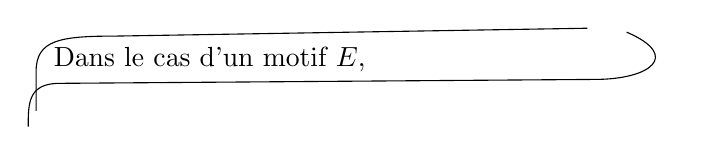
\begin{tikzpicture}[x=1cm,y=1cm]
\draw (0,0)--(0,0.5).. controls (0,0.9) and (0.3,0.95)..(1,0.95)--(7,1.05);\draw (7.5,1).. controls (8.2,0.7) and (7.8,0.4)..(7.1,0.4)--(0.3,0.35).. controls (-0.1,0.35) and (-0.1,0.1)..(-0.1,-0.2);
\node[anchor=west] at (0.1,0.65) {Dans le cas d'un \uline{motif} $E$,};
\end{tikzpicture}}
\unsure{Si} on exprime $\delta(E)$ et $\chi(E)$ en termes des \deleted{\unsure{ses}} composantes virtuelles de $\mathbf R f_!(E)$ (utilisant conj. de Weil), on trouve
\[
\left\{\begin{aligned}
\chi(E)&=\sum(-1)^i\beta_i(E)\\
\delta(E)&=\prod_i\delta(h_!^i(E))^{(-1)^i}
\end{aligned}\right.
\]
\margin{$\beta_i(E)$ les \unsure{nbs|nbres} de Betti virtuels à coeff. dans $E$}

Or $h_!^i(E)$ donne $\beta_i$ valeurs propres de val. absolue $p^{i/2}$, donc
\[\deleted{\unsure{\delta(E)=}}\delta(h_!^i(E))=\varepsilon_i p^{\frac{i\beta_i}{2}}\]
\margin{(NB. $i\beta_i/2$ : tjrs entier)}
où \deleted{$\unsure{\delta}$} $\varepsilon_i$ est défini comme un signe de discriminant virtuel, et c'est \deleted{$\unsure{\varepsilon}$} $+1$ si $i$ est impair. On trouve alors
\[
\left\{\begin{aligned}
\delta(E)&=\deleted{\unsure{\varepsilon(E)p^{\frac12\sum_i i\beta_i}}}\varepsilon(E)p^{\frac12\sum_i(-1)^i i\beta_i(E)}\\
\varepsilon(E)&=\prod_i\varepsilon_i(E)
\end{aligned}\right.
\]
\margin{$\varepsilon(E)$ et les $\varepsilon_i(E)$ sont $\pm1$, $\varepsilon_i(E)=+1$ si $i$ impair.}
\mspage{22}
\scanpage{24}
\begin{center}6 - 42 -\end{center}
\hfill n° 392

2) Les hypothèses sur $A$ et $B$ étant les mêmes que dans l'exerc. 1, soit $C$ un anneau tel que $A\subset C\subset B$ et que le corps des fractions de $C$ soit égal à $L$ ; tout idéal $\neq0$ dans $C$ est alors un \uline{réseau} de $L$, (relativement à $A$).

a) Montrer que si $\uline{a}$, $\uline{b}$ sont deux idéaux de $C$ tels que $\uline{a}$ soit pseudo-inversible, on a $\chi(\uline{ab},C)=\chi(\uline{a},C)+\chi(\uline{b},C)$.

b) On dit que deux idéaux $\uline{a}$, $\uline{b}$ de $C$ sont \uline{pseudo-étrangers} si, pour tout idéal premier $\uline{p}$ de hauteur 1 dans $A$, $\uline{a}_{\uline{p}}$ et $\uline{b}_{\uline{p}}$ sont étrangers dans $C_{\uline{p}}$. Montrer que si $\uline{a}$ et $\uline{b}$ sont pseudo-étrangers et $\neq0$, on a $\chi(\uline{ab},C)=\chi(\uline{a},C)+\chi(\uline{b},C)$. (Se ramener au cas où $A$ est un anneau de valuation discrète, observer que l'on a $\chi(\uline{a},\uline{a}+\uline{b})=\chi(\uline{a}\cap\uline{b},\uline{b})$ et utiliser la relation (\quad) du n°\quad du § 4).

c) Déduire de b) que si $\uline{a}$ est un idéal $\neq0$ de $C$, et si $\uline{q}_i$, $(1\leq i\leq r)$, sont les idéaux primaires de la décomposition primaire réduite de $\uline{a}$, correspondant aux idéaux premiers non immergés, on a $\chi(\uline{a},C)=\sum_i\chi(\uline{q}_i,C)$.

d) Soient $\uline{q}$ un idéal primaire de $C$, $\uline{p}$ l'idéal premier correspondant. Si $\uline{p}$ n'est pas de hauteur 1, on a $\chi(\uline{q},C)=0$ ; dans le cas contraire, si $\uline{p}_0=\uline{p}\cap A$, on a $\chi(\uline{q},C)=\deg_A(\uline{q})\cdot\uline{p}_0$.

e) Soit $\uline{a}$ un idéal de $C$ ; pour que $\uline{a}$ soit pseudo-inversible, (exerc. 1 b)), il faut et il suffit que l'on ait $\chi(\uline{a},C)=\chi(\uline{a}B,B)$. (Même méthode que dans l'exerc. 1 b)).

3) Les hypothèses sur $A$, $B$ et $C$ sont les mêmes que dans l'exerc. 2. On dit encore que le réseau $C^*$ est la \uline{codifférente} de $C$, et que $C:C^*$, qui est un idéal de $C$, est la \uline{différente} de $C$ sur $A$ ; on la note $\uline{D}_{C/A}$.

a) Montrer que le \uline{conducteur} $\uline{f}_{C/B}$ de $B$ dans $C$, (chap. V, § 1, n°\quad), est égal à $B^*:C^*$, et que pour tout idéal premier $\uline{p}$ de hauteur 1 dans $A$, on a $(\uline{f}_{C/B})_{\uline{p}}C^*_{\uline{p}}=B^*_{\uline{p}}$, (utiliser le fait que $B_{\uline{p}}$ est un anneau principal).

b) Montrer que l'on a $\uline{D}_{C/A}\subset\uline{f}_{C/B}\cap\uline{D}_{B/A}$, (utiliser a)).

c) Montrer que, pour que $C^*$, considéré comme idéal fractionnaire de $C$, soit pseudo-inversible, (exerc. 1 b)), il faut et il suffit que pour tout idéal premier $\uline{p}$ de hauteur 1 dans $A$, on ait $B_{\uline{p}}(\uline{D}_{C/A})_{\uline{p}}=(\uline{f}_{C/B})_{\uline{p}}(\uline{D}_{B/A})_{\uline{p}}$, (utiliser a)).

d) Si $C^*$ est pseudo-inversible, tout idéal fractionnaire $\uline{a}\neq0$ de $C$ tel que $\uline{a}:\uline{a}=C$ est pseudo-inversible, (utiliser le fait que pour deux idéaux fractionnaires non nuls $\uline{a}$, $\uline{b}$ de $C$, on a $(\uline{ab})^*=\uline{a}^*:\uline{b}$).
\mspage{23}
\scanpage{25}
Comparaison générale de $\unsure{L_E^\infty|L_E^-}$ et $L_{DE}^\infty$
\[\deleted{\unsure{\mathbf R i_*E}\mathbf R\bar f_*j^*\mathbf R i_*(E)}\]
\diagram{\begin{tikzcd}[ampersand replacement=\&,column sep=0.15em,row sep=1.1em]
\mathbf R_\infty f(E)=\mathbf R\bar f_*j^* \& \underbrace{(\mathbf R i_*(E))}\arrow[d,no head]\\
D\mathbf R_\infty f(E)=D\mathbf R\bar f_* \& (\qquad)
\end{tikzcd}}
\[
\begin{aligned}
&=\mathbf R\bar f_*D(\qquad)\\
&=\mathbf R\bar f_*\mathbf R j^!(D\mathbf R i_*(E))
\end{aligned}
\quad\left.\vphantom{\begin{matrix}1\\1\\1\end{matrix}}\right\}\quad\text{\uuline{dualité locale}}
\]
\[=\mathbf R\bar f_*\left(\mathbf R j^!\left(\mathbf R i_!(D(E))\right)\right)\]
\diagram{\begin{tikzcd}[row sep=0.4em]
\underbrace{\mathbf R j^!(\mathbf R i_!(D(E)))}\arrow[d,no head]\\
j^*(\mathbf R i_*(D(E)))[1]
\end{tikzcd}}
\[\boxed{D\mathbf R_\infty^*f(E)=\mathbf R_\infty^*(f(D(E)))[1]}\]
\margin{à vérifier si c'est $1$ ou $-1$ !}
\diagram{\begin{tikzcd}[row sep=0.5em]
\deleted{\boxed{\unsure{L_E^\infty(t)L_E^\infty(t)=1}}}\arrow[d]\\
\inserted{L_{DE}^\infty}
\end{tikzcd}}
\deleted{Supposons $\uline{D(E)}\simeq\unsure{\check E|E}(n+\rho)$, on trouve}

Supposons $E$ loc. ct. \inserted{de poids $\rho$} et $X$ lisse de dim \unsure{rel. $n$} \unsure{partout|pure}, on \unsure{trouve}
\[D(E)\simeq\check E(n)\simeq E(n+\rho)\]
d'où
\[\boxed{D\mathbf R_\infty^*f(E)\simeq\mathbf R_\infty^*f(E)(n+\rho)\unsure{*|+}[1]}\]
donc on a l'équation fonctionnelle
\[(-t)^{-\chi_\infty(E)}\delta_\infty(E)L_E^\infty(t^{-1})=L_E^\infty\left(p^{-(n+\rho)}t\right)^{-1}\]
i.e.
\[\boxed{L_E^\infty\left(\frac1{p^{(n+\rho)}t}\right)\underbrace{L_E^\infty(t)}(-t)^{\chi_\infty(E)}\delta_\infty(E)=1}\]
\mspage{24}
\scanpage{26}
\hfill Rédaction n° 397
\begin{center}
COMPLÉMENTS AU CHAPITRE VII D'ALGÈBRE

DUALITÉ DES MODULES DE LONGUEUR FINIE SUR UN ANNEAU PRINCIPAL

-:-:-:-
\end{center}

1. \uline{Modules injectifs}.

DEFINITION 1.- \uline{Soit} $A$ \uline{un anneau}, \uline{et soit} $I$ \uline{un} $A$-\uline{module}. \uline{On dit que} $I$ \uline{est injectif si}, \uline{pour toute suite exacte} $E'\longrightarrow E\longrightarrow E''$ \uline{d'applications} $A$-\uline{linéaires}, \uline{la suite} :
\[\operatorname{Hom}(E'',I)\longrightarrow\operatorname{Hom}(E,I)\longrightarrow\operatorname{Hom}(E',I)\]
\uline{est exacte}.

PROPOSITION 1.- \uline{Soit} $I$ \uline{un} $A$-\uline{module}. \uline{Les conditions suivantes sont équivalentes} :

(i) $I$ \uline{est injectif}.

(ii) \uline{Pour tout homomorphisme injectif} $F\longrightarrow G$, \uline{l'homomorphisme correspondant} $\operatorname{Hom}(G,I)\longrightarrow\operatorname{Hom}(F,I)$ \uline{est surjectif}.

Posons, pour simplifier l'écriture, (et pour tricher un peu !) :
\[D(F)=\operatorname{Hom}(F,I).\]
La condition (ii) signifie que, si $0\longrightarrow F\longrightarrow G$ est une suite exacte, la suite :
\[D(G)\longrightarrow D(F)\longrightarrow0\]
est exacte. On voit bien qu'elle est entraînée par (i).

Inversement, supposons (ii) vérifiée, et soit $E'\longrightarrow E\longrightarrow E''$ une suite exacte quelconque. Considérons la décomposition canonique de cette suite, (cf. Alg. II, 3e édition, p. 21) :
\diagram{\begin{tikzcd}[ampersand replacement=\&,row sep=0.7em,column sep=1em]
\& E'\arrow[r] \& S\arrow[r] \& 0 \& \\
0\arrow[r] \& S\arrow[r] \& E\arrow[r] \& T\arrow[r] \& 0\\
\& 0\arrow[r] \& T\arrow[r] \& E''. \&
\end{tikzcd}}
\mspage{25}
\scanpage{27}
\uline{NB}
\[\chi_\infty(E)=\varepsilon(\mathbf R f_*(E))-\varepsilon(\mathbf R f_!(E))\]
Or on a vu que les deux $\varepsilon$ sont égaux, donc $\chi_\infty(E)=0$. De même on a
\[\delta_\infty(E)=\delta(\mathbf R f_*(E))\delta(\mathbf R f_!(E))^{-1}\]
et on a vu que
\[p^{(n+\rho)\chi(E)}\delta(\mathbf R f_*(E))^{-1}=\delta(\mathbf R f_!(E))\]
d'où
\[\left\{\begin{aligned}
\delta_\infty(E)&=p^{(n+\rho)\chi(E)}\delta(E)^{-2}=\varepsilon(E)^{-2}\quad\deleted{\unsure{\delta(E)^2p^{-(n+\rho)\chi(E)}}}\\
\varepsilon(E)&=\delta(E)p^{-(n+\rho)\chi(E)/2}
\end{aligned}\right.\]
\margin{($=\pm1$ si $X$ est \deleted{\unsure{complet}} propre)}
(qui est bien $1$ lorsque $X$ est complet !)

d'où l'équation fonctionnelle
\[\boxed{L_E^\infty\left(\frac1{p^{n+\rho}t}\right)L_E^\infty(t)\delta_\infty(E)=1}\]
\[\left(\delta_\infty(E)=p^{(n+\rho)\chi(E)}\delta(E)^{-2}\deleted{\unsure{\delta}}=\varepsilon(E)^{-2}\right)\]

[Invariants arithmétiques équivalents,

(moyennant la connaissance de l'invariant \uline{géométrique} $\chi(E)$, et de $q=\deleted{\unsure{p}}p^{n+\rho}$)
\margin{\fbox{\parbox{3.1cm}{\uline{NB}. $\varepsilon(E)=\pm1$ si $X$ complet}}}
\[\delta(E)=\delta_!^*(E),\quad\delta'(E)=\unsure{\delta_*^*(E)|\delta_\cdot^*(E)},\quad\varepsilon(E),\quad\delta_\infty(E)\]
]
\[\boxed{\delta(E)\delta'(E)=q^{\chi(E)}}\]
\[\boxed{\varepsilon(E)=\delta(E)q^{-\chi(E)/2}=\delta'(E)q^{-\chi(E)/2}}\]
\margin{\figure{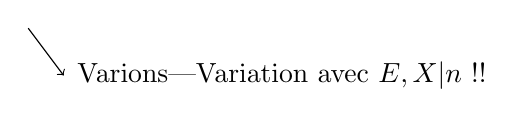
\begin{tikzpicture}[x=1cm,y=1cm]\draw[->] (0,0.6)--(0.45,0);\node[anchor=west] at (0.5,0) {\unsure{Varions|Variation} avec $E,\unsure{X|n}$ !!};\end{tikzpicture}}}
\[\boxed{\begin{aligned}
\delta_\infty(E)&=q^{\chi(E)}\delta(E)^{-2}=q^{-\chi(E)}\delta'(E)^{\unsure{2}}\\
&=\varepsilon(E)^{-2}
\end{aligned}}\]
\mspage{26}
\scanpage{28}
\begin{center}4 - 22 -\end{center}
\hfill n° 392

PROPOSITION 10.- (i) \uline{Soit} $0\longrightarrow T_1\longrightarrow T_2\longrightarrow T_3\longrightarrow0$ \uline{une suite exacte de} $A$-\uline{modules de torsion de type fini}. \uline{On a alors} :
\[\chi(T_2)=\chi(T_1)+\chi(T_3).\]
(ii) \uline{S'il existe un pseudo-isomorphisme} $f:T_1\longrightarrow T_2$, \uline{on a} $\chi(T_1)=\chi(T_2)$.

(iii) \uline{Pour que} $\chi(T)=0$, \uline{il faut et il suffit que} $T$ \uline{soit pseudo-nul}.

Vu la déf. 4, il suffit de considérer pour chaque $\uline{p}\in P$, les valeurs de $\ell_{\uline{p}}$ pour les modules de torsion considérés. La propriété (i) résulte alors du chap. II, § 2, n° 4, th. 1 et de l'additivité des longueurs dans une suite exacte, (\uline{Alg.}, chap. II, 3e éd., § 1, n° 10, prop. 16), et les propriétés (ii) et (iii) résultent aussitôt des définitions du n° 4.

COROLLAIRE.- \uline{Soit} $0\longrightarrow T_n\longrightarrow T_{n-1}\longrightarrow\cdots\longrightarrow T_0\longrightarrow0$ \uline{une suite exacte de} $A$-\uline{modules de torsion de type fini}. \uline{On a} $\sum_{i=0}^n(-1)^i\chi(T_i)=0$.

Vu le chap. II, § 2, n° 4, th. 1, cela résulte encore de la propriété analogue des $\ell_{\uline{p}}$, (\uline{Alg.}, chap. II, 3e éd., § 1, n° 10, cor. 3 de la prop. 16).

Rappelons, (chap. II, § 5, n° 4), que l'on peut parler de \uline{l'ensemble} $\uline{F}(A)$ \uline{des classes de} $A$-\uline{modules de type fini} pour la relation d'isomorphie pour tout $A$-module $M$ de type fini, on désigne par $c\ell(M)$ l'élément correspondant de $\uline{F}(A)$ ; nous désignerons par $\uline{T}(A)$ la partie de $\uline{F}(A)$ formée des classes de $A$-modules de torsion de type fini. Il est clair que $\chi$ définit une application de $\uline{T}(A)$ dans $D(A)$, notée encore $\chi$, telle que $\chi(c\ell(T))=\chi(T)$.

PROPOSITION 11.- \uline{Soient} $G$ \uline{un groupe commutatif}, \uline{noté additivement}, \uline{et} $\varphi:\uline{T}(A)\longrightarrow G$ \uline{une application} ; \uline{pour tout} $A$-\uline{module de torsion de type fini} $T$, \uline{on pose encore}, \uline{par abus de langage}, $\varphi(T)=\varphi(c\ell(T))$. \uline{On suppose vérifiées les conditions suivantes} :

1) Si $0\longrightarrow T_1\longrightarrow T_2\longrightarrow T_3\longrightarrow0$ \uline{est une suite exacte de} $A$-\uline{modules de torsion de type fini}, \uline{on a} $\varphi(T_2)=\varphi(T_1)+\varphi(T_3)$.
\mspage{27}
\scanpage{29}
Comparons cette équation fonctionnelle avec celle pour la fonction $L_E$, on trouve, en \deleted{\unsure{substituant}} posant pour simplifier $p^{n+\rho}=q$, et $A(t)\delta(E)(-t)^{\chi(E)}=B(t)$ :
\[
L\left(\frac1{qt}\right)=B(t)L(t)
\]
et faisant $t\mapsto\frac1{qt}$ dedans, on trouve
\[
L(t)=B\left(\frac1{qt}\right)L\left(\frac1{qt}\right)=B\left(\frac1{qt}\right)B(t)L(t)
\]
d'où
\[
B(t)B\left(\frac1{qt}\right)=1.
\]
Remplaçant $B$ par sa valeur, on trouve
\[
L_E^\infty\left(\frac1{\deleted{\unsure{p^{n+\rho}}}qt}\right)^{-1}\delta(E)(-t)^{\chi(E)}L_E^\infty(t)^{-1}\delta(E)\left(\frac{-1}{qt}\right)^{\chi(E)}=1
\]
i.e.
\[
\deleted{\unsure{L_E^\infty(\frac1{p^{n+\rho}t})^{-1}|L_E^\infty(p^{n+\rho}t)}}
\qquad L_E^\infty(t)L_E^\infty\left(\frac1{qt}\right)=\delta(E)^2\deleted{\frac1q}q^{-\chi(E)}.
\]
C'est précisément l'équation fonctionnelle explicitée plus haut.

Posons
\[
\unsure{\xi|\zeta}_E(t)=t^{\chi(E)/2}L_E(t)
\]
alors
\[
\begin{aligned}
\unsure{\xi|\zeta}_E\left(\frac1{qt}\right)&=\left(\frac1{qt}\right)^{\chi(E)/2}L_E\left(\frac1{qt}\right)=\left(\frac1{qt}\right)^{\chi(E)/2}A(t)\delta(E)(-t)^{\chi(E)}L_E(t)\\
&=\underbrace{q^{-\chi(E)/2}A(t)\delta(E)}(-1)^{\chi(E)}\underbrace{t^{\chi(E)/2}L_E(t)}_{\unsure{\xi|\zeta}_E(t)}
\end{aligned}
\]
i.e.
\mspage{28}
\scanpage{30}
\begin{center}6 - 41 - \hfill n° 392

\S 5.\end{center}
1) Soient $A$ un anneau noethérien intégralement clos, $K$ son corps des fractions, $L$ une extension de degré $n$ de $K$, $B$ la fermeture intégrale de $A$ dans $L$ ; on suppose que $B$ est un $A$-module de type fini. Soient $E$, $F$ deux anneaux tels que $A\subset E\subset F\subset B$.

a) Montrer que pour tout idéal premier $\uline{p}$ de hauteur 1 dans $E$, il n'y a qu'un nombre fini d'idéaux premiers $\uline{P}$ de $F$ au-dessus de $\uline{p}$ et qu'ils sont de hauteur 1 ; réciproquement, pour tout idéal premier $\uline{P}$ de hauteur 1 dans $F$, $\uline{P}\cap E$ est de hauteur 1 dans $E$.

b) Pour tout idéal premier $\uline{P}$ de hauteur 1 dans $F$, on appelle \uline{degré} de $\uline{P}$ par rapport à $E$, et on note $\deg_E(\uline{P})$ le degré du corps des fractions de $F/\uline{P}$ sur le corps des fractions de $E/(\uline{P}\cap E)$ ; le degré par rapport à $E$ d'un idéal premier de $F$ qui n'est pas de hauteur 1 est pris égal à 0 par définition. Si $\uline{Q}$ est un idéal primaire de $F$, $\uline{P}$ l'idéal premier correspondant, et si $m$ est le plus petit entier tel que la puissance symbolique $\uline{P}^{(m)}$ de $\uline{P}$ soit contenue dans $\uline{Q}$, on pose $\deg_E(\uline{Q})=m.\deg_E(\uline{P})$, (de sorte que $\deg_F(\uline{Q})=m$ si $\uline{P}$ est de hauteur 1, $\deg_F(\uline{Q})=0$ dans le cas contraire). Finalement, si $\uline{a}$ est un idéal quelconque $\ne0$ de $F$, $\uline{Q}_i$ les idéaux primaires de la décomposition primaire réduite de $\uline{a}$, correspondant aux idéaux premiers non immergés, on pose $\deg_E(\uline{a})=\sum_i\deg_E(\uline{Q}_i)$.

Avec ces notations, soit $C$ un anneau tel que $A\subset C\subset B$ ; on dit qu'un idéal $\uline{a}$ de $C$ est \uline{pseudo-inversible} si, pour tout idéal premier $\uline{p}$ de hauteur 1 dans $A$, $\uline{a}_{\uline{p}}$ est inversible dans l'anneau semi-local $C_{\uline{p}}$. Montrer que, pour que $\uline{a}\ne0$ soit pseudo-inversible, il faut et il suffit que l'on ait $\deg_C(\uline{a})=\sum_{\uline{P}}n(\uline{P})\deg_C(\uline{P})$, où $\uline{P}$ parcourt l'ensemble des idéaux premiers de hauteur 1 de $B$ et les $n(\uline{P})$ sont définis par $\operatorname{div}(\uline{a}B)=\sum_{\uline{P}}n(\uline{P})\uline{P}$. (Se ramener au cas où $A$ est un anneau de valuation discrète, donc $C$ semi-local. Observer d'une part que dans $C$, il y a alors identité entre les idéaux inversibles et les idéaux principaux, et que si $\uline{a}=xC$, $\deg_C(\uline{a})$ est égal à la longueur du $C$-module $C/xC$, et aussi à celle du $C$-module $B/xB$. D'autre part, si $\uline{m}_i$, $(1\le i\le r)$, sont les idéaux maximaux distincts de $C$, $\uline{a}\ne0$ un idéal de $C$, il existe $y\in\uline{a}$ tel que $y\notin C\cap(\uline{a}\uline{m}_iB)$ pour tout $i$ ; en déduire que $yB=\uline{a}B$, en utilisant le fait que $B$ est alors un anneau principal).
Si $C=B$, tout idéal $\ne0$ de $B$ est pseudo-inversible.
\mspage{29}
\scanpage{31}
\[
\boxed{\unsure{\xi|\zeta}_E\left(\frac1{qt}\right)=A^{\unsure{\xi}}(t)\varepsilon'(E)\unsure{\xi|\zeta}_E(t)}
\qquad q=p^{n+\rho}
\]
\figure{\begin{tikzpicture}[x=1cm,y=1cm]\draw (0,0.8) .. controls (-.25,.7) and (.2,.45) .. (0,.3) .. controls (-.15,.15) and (.25,-.3) .. (.03,-.4);\end{tikzpicture}}
\[
\left\{\begin{aligned}
A(t)&=L_E^\infty\left(\frac1{qt}\right)^{-1}\\
\varepsilon'(E)&=\varepsilon(E)(-1)^{\chi(E)}
\end{aligned}\right.
\qquad \varepsilon(E)=\deleted{\unsure{\delta(E)p^{-(n+\rho)\chi(E)/2}}}\delta(E)q^{-\chi(E)/2}
\]
Si $\deleted{\unsure{E}}X$ \unsure{complète|complet}
\[
\left\{\begin{aligned}A(t)&=1\\\varepsilon'(E)&=\pm1.\end{aligned}\right.
\]
\mspage{30}
\scanpage{32}
\begin{center}6 - 40 - \hfill n° 392\end{center}
c) Si $\uline{e}(E)$ est un idéal principal $A\alpha$, montrer que $E$ contient un facteur direct isomorphe à $A/A\alpha$, (écrire $E$ comme quotient de $A^r$ par un sous-module $R$ et noter qu'il y a dans $R$ un élément de la forme $\alpha y$, où $y$ est un élément d'une base de $A^r$).

d) Soit $\uline{d}'_h(E)$ l'annulateur de $\bigwedge^{h+1}E$ pour $0\le h\le r-1$. Montrer que les conditions suivantes sont équivalentes :

$\alpha)$ Les idéaux $\uline{d}_h(E)$, $(0\le h\le r-1)$, sont principaux.

$\beta)$ Les idéaux $\uline{d}'_h(E)$, $(0\le h\le r-1)$, sont principaux.

$\gamma)$ $E$ est somme directe de $r$ modules isomorphes à $A/A\lambda_h$, où $\lambda_{h+1}$ divise $\lambda_h$ pour $0\le h\le r-1$.

En outre, lorsque ces conditions sont vérifiées, on a $\uline{d}'_h(E)=A\lambda_h$ pour $0\le h\le r-1$, et $\uline{d}_h(E)=\lambda_h\lambda_{h+1}\ldots\lambda_{r-1}A$ pour $0\le h\le r-1$. (Procéder par récurrence sur $r$, en utilisant c)).

e) On suppose en outre que $A$ est intègre. Montrer que si $\uline{p}$ est un idéal premier de $A$ tel que $E/\uline{p}E$ soit un $(A/\uline{p})$-module libre et $E_{\uline{p}}$ un $A_{\uline{p}}$-module libre, alors $E$ est un $A$-module libre, (en utilisant b), montrer que $\gamma(E_{\uline{p}})=\gamma(E)$ et que $\uline{e}(E_{\uline{p}})=\uline{e}(E)$).

23) Soient $A$ un anneau, $E$ un $A$-module de type fini, $r$ le plus petit des entiers $k$ tels que $\bigwedge^{r+1}E=0$, $\uline{e}(E)$ l'annulateur de $\bigwedge^rE$. Montrer que pour tout idéal $\uline{a}\supset\uline{e}(E)$ dans $A$, le $(A/\uline{a})$-module $E/\uline{a}E$ est plat, (se ramener au cas où $A$ est un anneau local, et utiliser l'exerc. 22 b)). En déduire que si $\uline{r}$ est le radical de $A$ et si, pour tout idéal maximal $\uline{m}$ de $A$, la dimension du $(A/\uline{m})$-espace vectoriel $E/\uline{m}E$ est la même, alors $E/\uline{r}E$ est un $(A/\uline{r})$-module plat.
\begin{center}-:-:-:-\end{center}
\mspage{31}
\scanpage{33}
Cas d'une courbe alg.

$X$ \inserted{courbe} lisse projective \inserted{[\unsure{irred}]} sur $\mathbb F_p$, \deleted{\unsure{lisse}} corps de fonctions $K$.
$E_y$ $\mathbb Q_\ell$-faisceau \unsure{constr.} sur $y=\operatorname{Spec}K$.

On veut lui associer une ``fonction L''. C'est raisonnable, car $K$ détermine $X$.

Prenons d'abord $E=i_*(E_y)$, où $i:y\unsure{-|\longrightarrow}X$.
On sait alors que
\[
D(E)=i_*(\check E_y)(1)
\]
\deleted{\unsure{Donc si on}} Donc si on pose
\[
L^*_{E_y}(t)=L_{i_*(E_y)}(t),
\]
on aura
\[
L^*_{\check E_y}\deleted{\unsure{(t)}}\left(\frac1{pt}\right)=(-t)^{\chi^*(\check E_y)}\delta^*(E_y)L^*_{E_y}(t).
\]
si on pose
\[
\begin{aligned}
\chi^*(E_y)&=\chi(i_*(E_y))\\
\delta^*(E_y)&=\delta(i_*(E_y))
\end{aligned}
\]
Supposons qu'on ait
\[
\check E_y=E_y(\rho)\qquad\text{d'où }i_*(\check E_y)=i_*(E_y)(\rho)
\]
alors on trouve ;
\[
\boxed{L^*_{E_y}\left(\frac1{qt}\right)=(-t)^{\chi^*(E_y)}\delta^*(E_y)L^*_{E_y}(t)}
\qquad(q=p^{1+\rho}
\]
\mspage{32}
\scanpage{34}
\begin{center}6 - 36 - \hfill n° 392\end{center}
g) Soient $K$ un corps, $A$ l'anneau de polynômes $K[X,Y,Z]$, $\uline{m}$ l'idéal maximal $AX+AY+AZ$, $\uline{q}$ l'idéal de $A$ engendré par $X$, $Y^2$, $YZ$ et $Z^2$. On considère le $A$-module $M=A/\uline{q}$ et son sous-module $N=\uline{m}/\uline{q}$. Montrer que l'on a $\uline{d}_0(M)=\uline{q}$, $\uline{d}_1(M)=A$, $\uline{d}_0(N)=\uline{m}^2$, $\uline{d}_1(N)=\uline{m}$.

11) Soient $A$ un anneau de Krull, $M$, $N$ deux réseaux de type fini dans un espace vectoriel $V$ de dimension finie $n$ sur le corps des fractions de $A$. Pour tout $c\ne0$ dans $A$ tel que $cN\subset M$, on considère les idéaux déterminantiels $\uline{d}_k(M/cN)$, (exerc. 10), et on pose :
\[
d_k(N,M)=\operatorname{div}(\uline{d}_k(M/cN))-(n-k)\operatorname{div}(c).
\]
a) Montrer que $d_k(N,M)$ ne dépend pas du choix de $c$ tel que $cN\subset M$ ; on dit que $d_k(N,M)$ est le \uline{diviseur déterminantiel} d'indice $k$ de $N$ par rapport à $M$.

b) On a $d_k(N,M)\ge d_{k+1}(N,M)$, et $d_n(N,M)=0$. Montrer que si l'on pose $e_k(N,M)=d_{n-k}(N,M)-d_{n-k+1}(N,M)$, on a $e_k(N,M)\le e_{k+1}(N,M)$ pour $1\le k\le n$ ; on dit que les diviseurs $e_k(N,M)$ sont les \uline{facteurs invariants} de $N$ par rapport à $M$, (se ramener au cas où $A$ est un anneau principal).

c) Montrer que l'on a $d_0(N,M)=\chi(M,N)$, (n° \quad).

d) Lorsque $M$ est un réseau dans $V$ mais que $N$ est un réseau dans un sous-espace $W$ de $V$ de dimension $q<n$, on appelle \uline{facteurs invariants} de $N$ par rapport à $M$ les facteurs invariants de $N$ par rapport à $M\cap W$. Montrer comment s'étendent les exerc. 8 à 10 et 14 à 16 d'\uline{Alg.}, chap. VII, § 4, (en supposant au besoin dans certains cas que $A$ est noethérien et intégralement clos).

12) Soient $A$ un anneau noethérien intégralement clos, $M$, $N$ deux $A$-modules sans torsion de type fini, de même rang $r$, tels que $N\subset M$ ; soit $j:N\longrightarrow M$ l'injection canonique.

a) Montrer que, pour tout $K$, $\bigwedge^k j:\bigwedge^kN\longrightarrow\bigwedge^kM$ est pseudo-injectif, que $\operatorname{Coker}(\bigwedge^k j)$ est un $A$-module de torsion et que l'on a :
\[
\chi(\operatorname{Coker}(\bigwedge^k j))=\binom{r-1}{k-1}\chi(\operatorname{Coker}j).
\]
b) En utilisant a), démontrer que si $M$ est un $A$-module sans torsion de type fini, le sous-module de torsion de $\bigwedge^kM$ est pseudo-nul pour tout $k$, et l'on a $c(\bigwedge^kM)=\binom{r-1}{k-1}c(M)$, où $M$ est de rang $r$ ; en particulier, on a $c(\bigwedge^rM)=c(M)$.
\mspage{33}
\scanpage{35}
Posant
\[
\unsure{\xi|\zeta}^*_{E_y}(t)=t^{\chi^*(E_y)/2}L^*_{E_y}(t)
\]
on trouve
\[
\boxed{\unsure{\xi|\zeta}^*_{E_y}\left(\frac1{qt}\right)=\varepsilon'{}^*(E_y)\unsure{\xi|\zeta}^*_{E_y}(t)}
\]
\[
\left\{\begin{aligned}
\varepsilon'{}^*(E_y)&=\delta^*(E_y)q^{-\chi^*(E_y)/2}(-1)^{\chi^*(E_y)}\\
q&=p^{1+\rho}
\end{aligned}\right.
\]
\unsure{ceci avec les}

\uline{Un reproche à faire à} $L^*_{E_y}(t)$ : \uline{ce n'est pas} \uline{additif} en $E$. De façon précise, si on a
\diagram{\begin{tikzcd}[ampersand replacement=\&]0\arrow[r]\&E'_y\arrow[r,dash]\&E_y\arrow[r,dash]\&E''_y\arrow[r,dash]\&0\end{tikzcd}}
On en conclut
\diagram{\begin{tikzcd}[ampersand replacement=\&]0\arrow[r,dash]\&i_*(E'_y)\arrow[r,dash]\&i_*(E_y)\arrow[r]\&\unsure{i_y^*|i_*}(E''_y)\arrow[r]\&Q\arrow[r]\&0\end{tikzcd}}
où
\figure{\begin{tikzpicture}[x=1cm,y=1cm]
\node[anchor=west] at (0,1.6) {$Q\deleted{=\operatorname{Ker}\bigl(R^1i_*(E'_y)-R^1i_*(E_y)\bigr)}$};
\node[anchor=west] at (.5,.15) {$\inserted{=\coprod_{\substack{x\ \text{pt ramifié}\\\text{de }E''_y}}\unsure{j_x\longleftarrow X}}$};
\draw (.7,1.3) .. controls (.7,.8) and (1,.6) .. (.7,.5) .. controls (.2,.4) and (.4,-.8) .. (1.2,-.85) -- (3.5,-.7) .. controls (4.6,-.6) and (4.7,-.15) .. (4.3,.2) -- (7.8,.3) .. controls (8.8,.4) and (8.7,.9) .. (9,1.6);
\draw (8.7,1.65) .. controls (8.1,1.9) and (8,1.2) .. (7.7,1.35) .. controls (6.8,1.9) and (6.1,.35) .. (5.5,.4) .. controls (4.7,.7) and (5.3,1.6) .. (4.7,1.25) .. controls (3.5,.1) and (3.1,.05) .. (2.7,.7);
\end{tikzpicture}}
est concentré \deleted{\unsure{aux}} \unsure{en un nb} fini de pts de ``ramification'' de $E''_y$.

D'où
\[
\left\{\begin{aligned}
L^*_{E_y}(t)&=L^*_{E'_y}(t)L^*_{E''_y}(t)L_Q(t)^{-1}=L^*_{E'_y}(t)L^*_{E''_y}(t)\prod_xP_{Q_x}(t)\\
Q_x&=\operatorname{Coker}(E_x-E''_x)
\end{aligned}\right.
\]
\margin{\figure{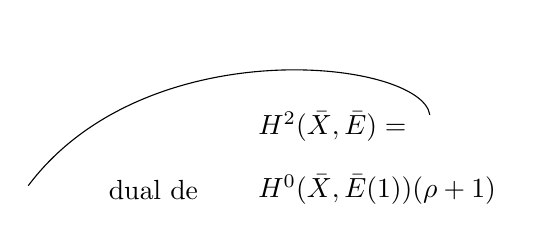
\begin{tikzpicture}[x=1cm,y=1cm]\draw (0,0) .. controls (1.5,2) and (5,1.6) .. (5.1,.9);\node[anchor=west] at (2.8,.75) {$H^2(\bar X,\bar E)=$};\node[anchor=west] at (.9,-.05) {dual de};\node[anchor=west] at (2.8,-.05) {$H^0(\bar X,\bar E\deleted{\unsure{(1)}})(\unsure{\rho+1})$};\end{tikzpicture}}}
\mspage{34}
